\section{Simulating and Reconstructing Tomography Data}

In this last section, we will go trough a series of practical experiments to, using the \textit{DeepInverse} library, to simulate and reconstruct tomography data.

The source code for this section can be seen in the Jupyter noteebok at the following link: \href{https://github.com/mhetacc/CIL/blob/6830cc50b972bd39f5c5c328295af87e33732a38/notebooks/CompleteCTlab.ipynb}{github/mhetacc/.../CT.ipynb}

\subsection{Model-Based Reconstruction}

The first objective is recovering an image $u$ from a set of noisy projections $y$. The measurements are modelled via the \textit{discrete Radon transform}
\begin{equation}
    \begin{aligned} \mathbf{y}(\boldsymbol{\theta},\rho) &= \int_{L_{\boldsymbol{\theta},\rho}}~u~d\sigma
    \end{aligned} \qquad \boldsymbol{\theta} \in \mathbb{R}^2,~ \| \boldsymbol{\theta}\|=1, \quad \rho \in \mathbb{R}_+
\end{equation}
where the collection of projections across all angles is called the \textit{sinogram}. 

Three acquisition geometries are studied: (i) \textit{full-angle} (180 projections), (ii) \textit{sparse-angle} (36 uniformly sampled angles), and (iii) \textit{limited-angle} (between 30 and 150 degrees). An example of the code for the definition of the forward model with 36 angles is shown in listing \ref{code:forward}.

\begin{lstlisting}[language=Python, label={code:forward}, caption={Defining the sparse-angle CT forward model with \textit{deepinv}.}]
import deepinv as dinv
import torch

theta_sparse = torch.tensor(
    np.linspace(0, 180, 36, endpoint=False)
).to(device)

tomo_sparse = dinv.physics.Tomography(
    angles=theta_sparse,
    img_width=128,
    circle=False,
    device=device
)

sinogram_sparse = tomo_sparse(u_SL_small)
\end{lstlisting}

Resulting sinograms can be seen in figure \ref{fig:sinograms}.

\begin{figure}[h]
    \centering
    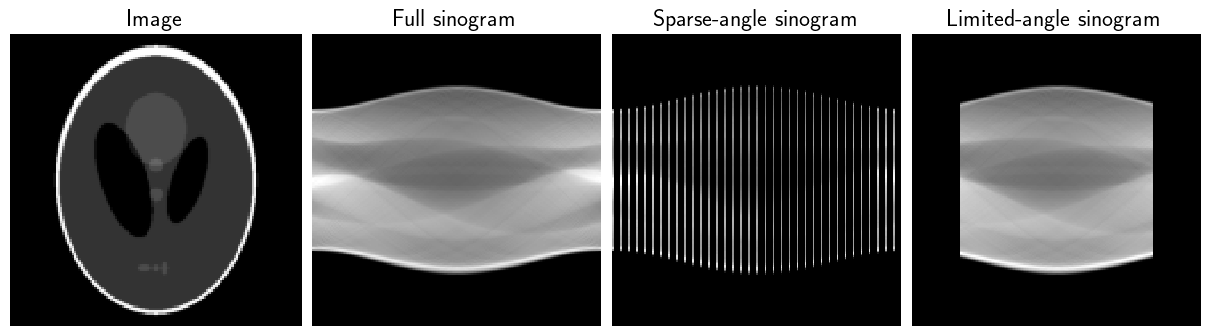
\includegraphics[width=.8\linewidth]{images/sinograms.png}
    \caption{Original image (on the left) and its sinograms under full-angle, sparse-angle, and limited-angle geometries.}
    \label{fig:sinograms}
\end{figure}

Gaussian noise is added to the sinogram via a custom class that scales the noise amplitude by $\max|x|$, making it signal-dependent (Listing~\ref{code:noise}).

\begin{lstlisting}[language=Python, label={code:noise}, caption={Custom Gaussian noise model for CT sinograms.}]
class GaussianNoiseCT(dinv.physics.GaussianNoise):
    def forward(self, x, sigma=None, seed=None, **kwargs):
        self.update_parameters(sigma=sigma, **kwargs)
        self.to(x.device)
        return (x + torch.max(torch.abs(x))
                * self.randn_like(x, seed=seed)
                * self.sigma[(...,) + (None,) * (x.dim()-1)])
\end{lstlisting}

\subsubsection{Näive inversion: Filtered Back-Projection}

An inverse problem can be representing as recovering $f$ from
$y = \text{noise}(A(u))$. When $A$ is linear, in the discrete formulation, this reduces to
\begin{equation}
    y = \mathbf{A} u + \epsilon, \quad u \in \mathbb{R}^n, \epsilon \in \mathbb{R}^m, \mathbf{A} \in \mathbb{R}^{m \times n}
\end{equation}

The simplest reconstruction strategy is to use \textit{Filtered Back-Projection} (FBP) to solve $u_{\text{naive}} = \mathbf{A}^{-1} y$. It is available directly from the physics object via \textit{tomo.fbp(sinogram)}. While fast, FBP is highly sensitive to noise and to incomplete angular coverage.

\subsubsection{Gradient Descent (unregularized)}

To avoid assembling the dense matrix $\mathbf{A}$, iterative solvers minimize $\frac{1}{2}\|\mathbf{A}u - y\|^2$ via gradient descent:
\begin{equation}
    \left\{
    \begin{aligned}
    u^{0} & \text{ given} \\
    u^{(k+1)} =&\  \mathbf{A}^T(\mathbf{A}u^{(k)}-y)
    \end{aligned}
    \right.
\end{equation}

In \textit{deepinv} this is assembled with \textit{optim\_builder} using a \textit{ZeroPrior} (example in listing \ref{code:gd}).

\begin{lstlisting}[language=Python, label={code:gd}, caption={Unregularised gradient descent reconstruction.}]
prior = dinv.optim.prior.ZeroPrior()

opt = dinv.optim.optim_builder(
    iteration="GD",
    prior=dinv.optim.prior.ZeroPrior(),
    data_fidelity=dinv.optim.data_fidelity.L2(),
    max_iter=100,
    crit_conv="residual",
    thres_conv=1e-4,
    early_stop=True,
    params_algo={"stepsize": 1.0}
)
u_hat, metrics = opt(y, tomo_exp, compute_metrics=True)
\end{lstlisting}

Results can be seen in figure \ref{fig:gradescent}.

\begin{figure}[h]
    \centering
    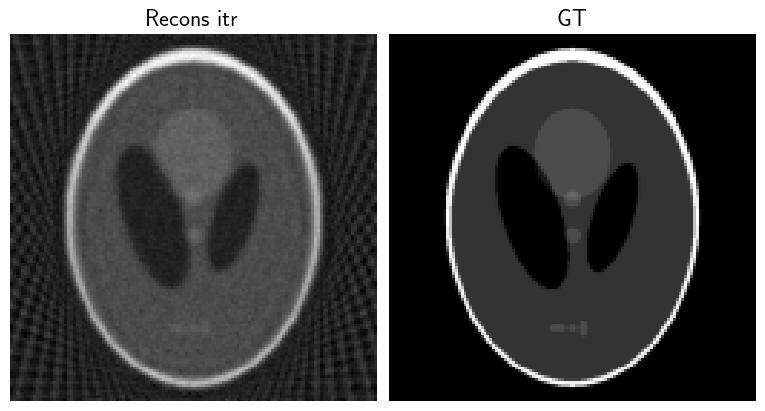
\includegraphics[width=.8\linewidth]{images/gradescent.png}
    \caption{Reconstruction with gradient method results.}
    \label{fig:gradescent}
\end{figure}

\subsubsection{Tikhonov Regularisation}

Penalizing large norms yields the \textit{Tikhonov} problem:
\begin{equation}
    u_\alpha^* = \arg\min_{u} \left\{ \tfrac{1}{2}\|\mathbf{A}u - y\|^2 + \alpha\|u\|^2 \right\}.
\end{equation}

but $u_\alpha^*$ can be found solving a linear system with symmetric, positive definite, matrix.
The first-order optimality condition gives $(\mathbf{A}^\top\mathbf{A} + \alpha I)u_\alpha^* = \mathbf{A}^\top y$, which is solved iteratively by replacing \textit{ZeroPrior} with \textit{dinv.optim.Tikhonov()} and setting \textit{"lambda": 0.1} in \textit{params\_algo}. The rest is similar to listing \ref{code:gd}.

\subsubsection{LASSO / Sparsity-Promoting Regularisation}

The lasso penalizes solutions with large $1$-norms, promoting solutions with few non-zero entries:
\begin{equation}
    u_\alpha^* = \arg\min_{u} \left\{ \tfrac{1}{2}\|\mathbf{A}u - y\|^2 + \alpha\|u\|_1 \right\}.
\end{equation}
This is solved by \textit{Proximal Gradient Descent} (PGD), where the proximal operator of $\alpha\|\cdot\|_1$ is soft-thresholding $S_\alpha(u) = \operatorname{sign}(u)(|u|-\alpha)^+$.

In code, we just have to \textit{iteration="PGD"} and \textit{prior=dinv.optim.L1Prior()}. 

The above algorithms need to be tuned with hyperparameters, for example \textit{step size}. We can visualize how the MSE, PSNR, and SSIM vary with different step sizes for the three algorithms. Results are shown in figure \ref{fig:msepsnrssim}. It is interesting to notice that, with \textit{deepinv} default $\lambda$ value, the zerio-prior algorithm seems to outperform the others.

\begin{figure}[h]
    \centering
    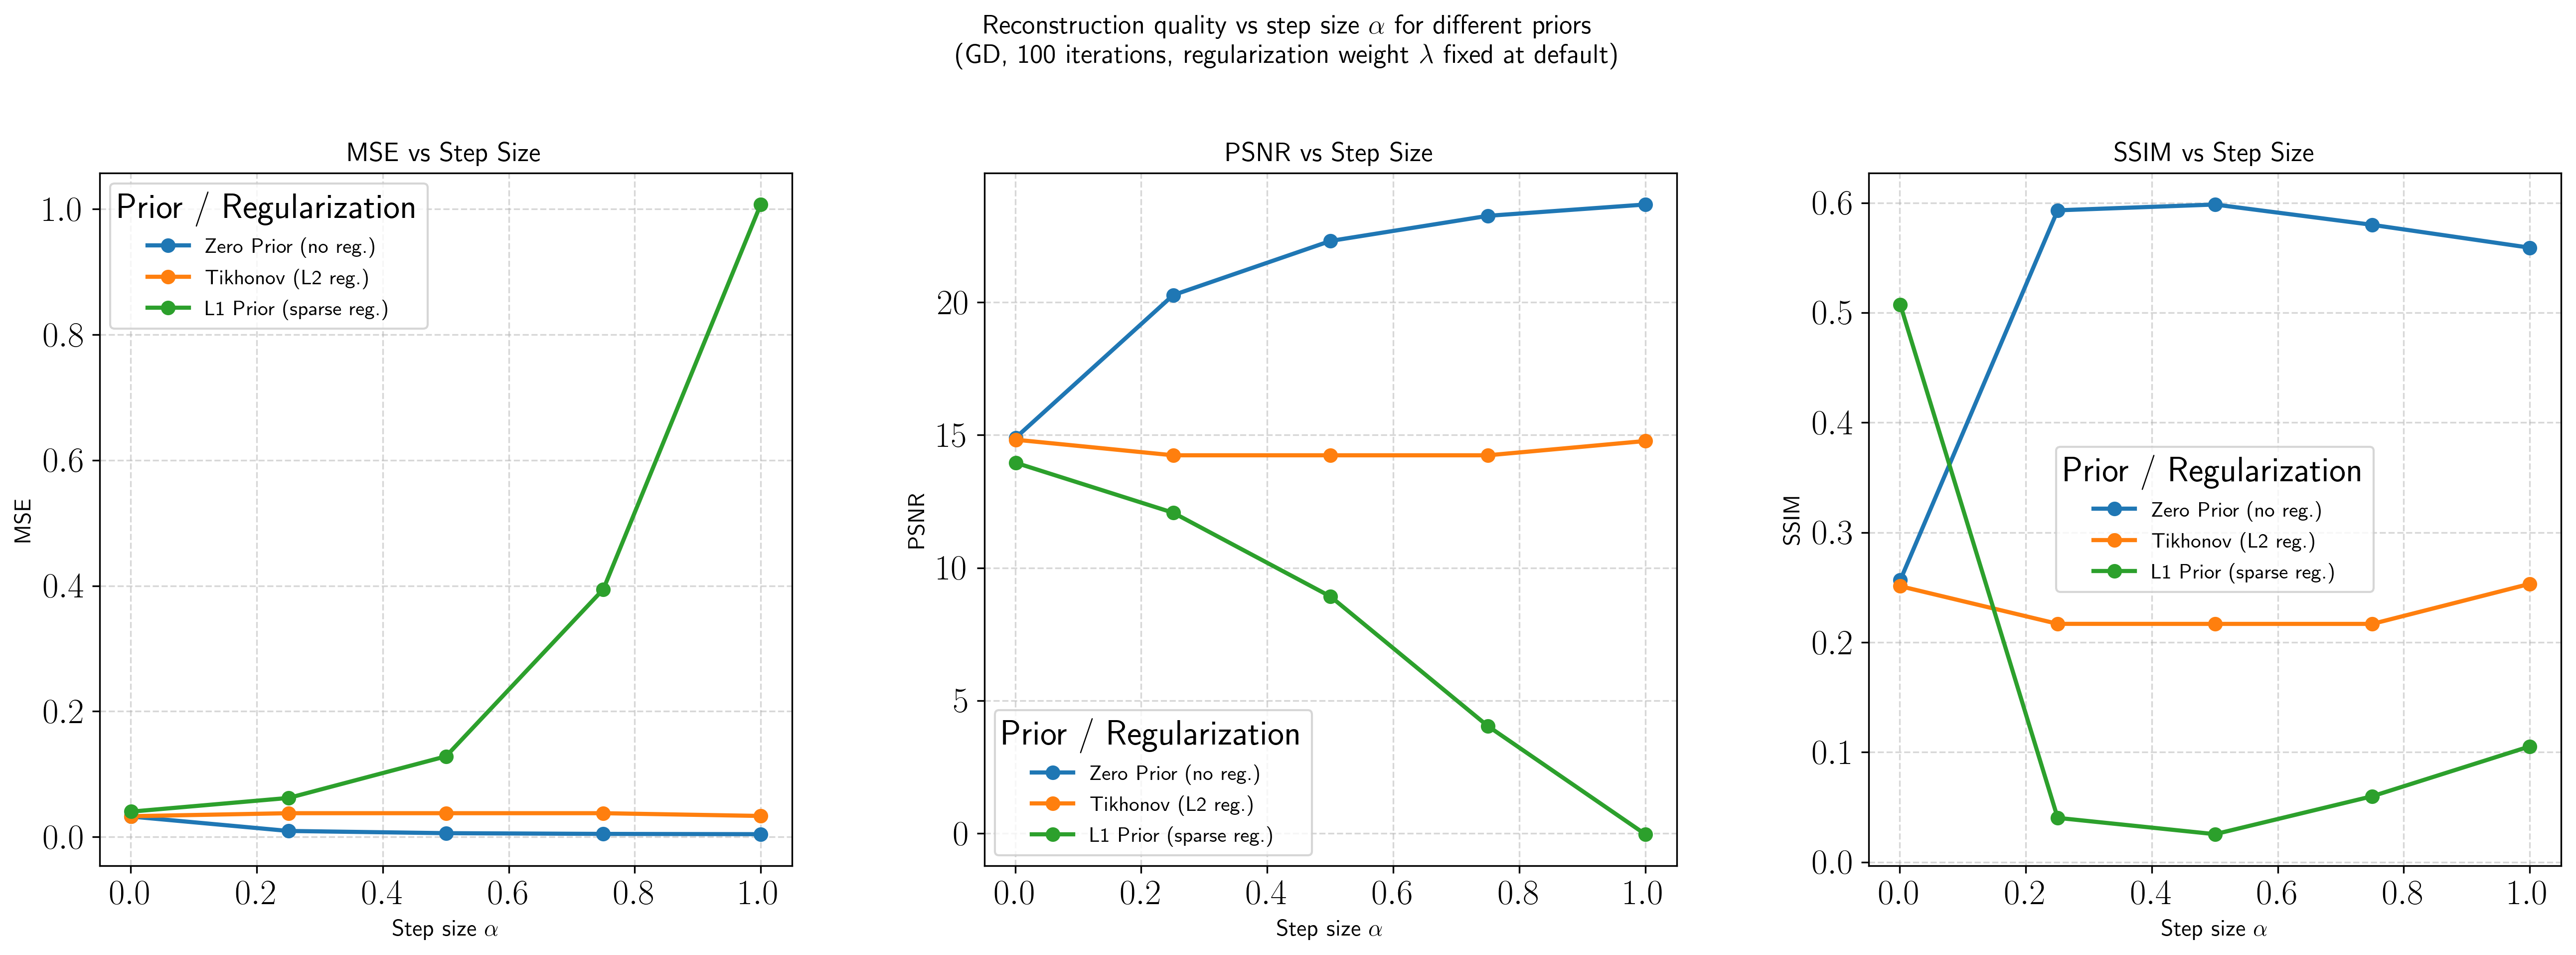
\includegraphics[width=\linewidth]{images/stepsizecompar.png}
    \caption{Hyperparameters comparison: MSE (left), PSNR (center), and SSIM (right).}
    \label{fig:msepsnrssim}
\end{figure}

\subsection{Learned Regularisation Functionals}
TODO

Up until this point we have seen how to solve the inverse problem using model-based reconstruction, by explicitly defining a regularization function that minimizes a cost function. While rigorous, hand-crafted priors are too static to capture complex and nuanced textures.  

We will now try to learn the \textit{regularisation functionals}. Instead of manually defining the regularizer, we will learn the prior distribution implicitly from data.

We will use the same class as before to add Gaussian noise, as well as a similar initialized module physics.


The first step is creating a supervised dataset by constructing $\{(y_i,u_i)\}_{i=1}^N$, where $u_i$ is an image from a dataset, specifically the MNIST datasets, taken from the \textit{datasets} module of the \textit{torchvision} library. We generate a dataset with two sub-datasets, one for training and one for testing, which is standard best practice.
Two samples from the dataset can be seen in figure \ref{fig:samples}.

\begin{figure}[h]
    \centering
    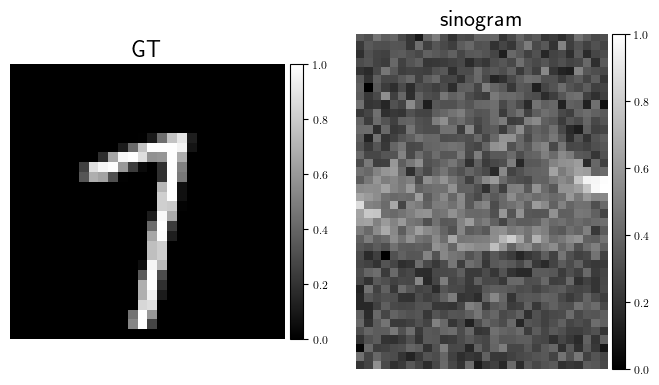
\includegraphics[width=.8\linewidth]{images/samplesdataset.png}
    \caption{Samples from train dataset constructed from MNIST. Ground truth on the left, sinogram on the right.}
    \label{fig:samples}
\end{figure}

First, we compute a reconstruction baseline with an L1 prior, step size of one and a lambda of $0.05$. We run the model builder for five hundred iterations to find and optimal solution. Results can be seen in figure \ref{fig:l1priorbaseline}.

\begin{figure}[h]
    \centering
    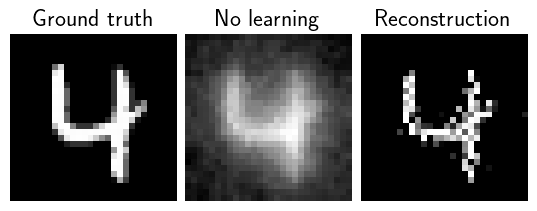
\includegraphics[width=.8\linewidth]{images/baselinel1.png}
    \caption{Baseline reconstruction with L1 prior, step size 1, lambda $0.05$ and 500 iterations.}
    \label{fig:l1priorbaseline}
\end{figure}

\subsection{Plug-and-Play with a Pre-trained Denoiser}

\textit{Plug-and-Play} (PnP) replaces the proximal step in PGD with a pre-trained denoising network $D_{\theta,\sigma}$, obtaining:
\begin{equation}
\left\{
    \begin{aligned}
        z^{(k+1)} &= u^{(k)} - \tau A^\top(Au^{(k)}-y) \\
        u^{(k+1)} &= D_{\theta,\sigma}(z^{(k+1)})
    \end{aligned}
\right.
\end{equation}

Now is the network itself that plays the role of denoiser, in particular it is trained to remove the Gaussian noise.

We first evaluate the results of a \textit{DnCNN} network pre-trained on natural images, directly available from the DeepInverse library of models. An example code is shown in listing \ref{code:dncnn}.

\begin{lstlisting}[language=Python, label={code:dncnn}, caption={PnP-PGD with a pre-trained DnCNN denoiser.}]
from deepinv.models import DnCNN

denoiser = DnCNN(in_channels=1, out_channels=1,
                 pretrained="download", device=device)
prior = PnP(denoiser=denoiser)

modelPnP = optim_builder(
    iteration="PGD",
    prior=prior,
    data_fidelity=dinv.optim.data_fidelity.L2(),
    early_stop=True,
    max_iter=200,
    params_algo={"stepsize": 0.8, "g_param": 0.1}
)
\end{lstlisting}

The resulting reconstruction leaves a lot to be desired, looking even worse than the baseline, as shown in figure \ref{fig:dncnn}.

\begin{figure}[h]
    \centering
    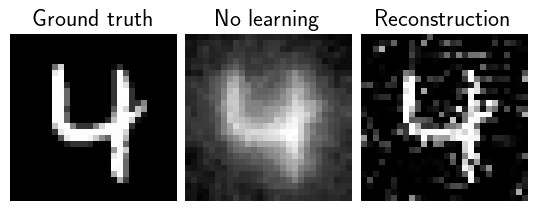
\includegraphics[width=.8\linewidth]{images/dncnndenoiser.png}
    \caption{Reconstruction with DnCNN pretrained on natural images as prior.}
    \label{fig:dncnn}
\end{figure}

\subsection{Training a Task-Specific Denoiser}

Now we want to train a \textit{DnCNN} denoiser specifically on the \textit{MNIST} dataset. 

First we create a new dataset $\{\tilde{u}_i,u_i\}_{i=1}^{N_{den}}$ such that $\tilde{u}_i = u_i + \tilde{\epsilon}_i$ where $\tilde{\epsilon}_i \sim \mathcal{N}(0,\sigma^2 I)$.

Then we define a denoiser $D_\theta$ and train it. We choose its parameters $\theta$ so to minimize
\begin{equation}
    L_{den}(\theta) = \frac{1}{N_{den}} \sum_{i=1}^{N_{den}} \| D_\theta(\tilde{u}_i) - u_i\|^2
\end{equation}

Finally, we use the trained denoiser in any PnP scheme.

Training uses \textit{dinv.Trainer} with the Adam optimiser for 20 epochs. The trained denoiser is then plugged into PnP-PGD and evaluated on the CT test set. An example code for the training can be seen in listing \ref{code:dncnntrain}.

\begin{lstlisting}[language=Python, label={code:dncnntrain}, caption={Training a DnCNN denoiser.}]
denoiser_train = DnCNN(in_channels=1, out_channels=1,
                pretrained="download",device=device,)
noise_model = dinv.physics.GaussianNoise(sigma=sigma_PnP)

trainer_den = dinv.Trainer(
    model=denoiser_train,
    physics=dinv.physics.Denoising(noise_model=noise_model),
    train_dataloader=DataLoader(train_dataset, batch_size=batch_size, num_workers=0, shuffle=False),
    eval_dataloader=DataLoader(test_dataset, batch_size=batch_size, num_workers=0, shuffle=False),
    epochs=20,
    losses=[dinv.loss.SupLoss(metric=dinv.loss.metric.MSE())],
    optimizer=torch.optim.Adam(denoiser_train.parameters(), lr=learning_rate),
    device=device,
)
\end{lstlisting}

Now that we have a trained denoiser, we can use it as prior to evaluate its performances. The results, shown in figure \ref{fig:pnptrained}, are satisfactory: the reconstructed image looks very close to the ground truth, and is a considerable improvement over our previous baseline.

\begin{figure}[h]
    \centering
    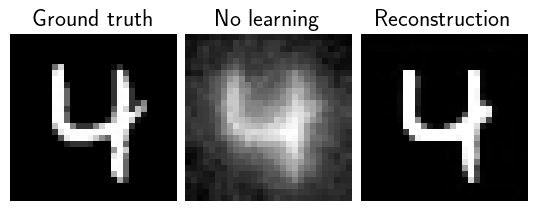
\includegraphics[width=.8\linewidth]{images/pnp_trained.png}
    \caption{Reconstruction with a DnCNN trained for the specific task. The resulting image is remarkably close to the ground truth, and improve significantly over the baseline.}
    \label{fig:pnptrained}
\end{figure}

\subsection{Summary}

The lab progressively builds from analytic inversion (FBP) to variational regularisation (Tikhonov, LASSO, TV) and finally to learned Plug-and-Play priors. Table~\ref{tab:methods} summarises the methods.

\begin{table}[h]
\centering
\caption{Summary of reconstruction methods explored in the lab.}
\label{tab:methods}
\begin{tabular}{lccc}
\hline
\textbf{Method} & \textbf{Algorithm} & \textbf{Prior}  \\
\hline
FBP             & Analytic           & None                 \\
GD (unregul.)   & Gradient Descent   & None                 \\
Tikhonov        & Gradient Descent   & Gaussian            \\
LASSO           & PGD                & Gaussian            \\
PnP (pretrained)& PGD                & Pretrained DnCNN     \\
PnP (trained)   & PGD                & Task-trained DnCNN   \\
\hline
\end{tabular}
\end{table}
